\documentclass[submit,techrep,noauthor]{ipsj}

\usepackage[dvips]{graphicx}
\usepackage{latexsym}

% bibtex用
\usepackage{url}

\def\Underline{\setbox0\hbox\bgroup\let\\\endUnderline}
\def\endUnderline{\vphantom{y}\egroup\smash{\underline{\box0}}\\}
\def\|{\verb|}

\begin{document}


\title{VoLP:声ラベルプリンタ 非同期音声コミュニケーション\\促進のためのIoTノードの提案}

\affiliate{TDU}{東京電機大学未来科学部情報メディア学科}
\author{橋本 慶紀}{Hashimoto Yoshiki}{TDU}[yoshiki@cps.im.dendai.ac.jp]
\author{岩井 将行}{Iwai Masayuki}{TDU}[iwai@cps.im.dendai.ac.jp]

\begin{abstract}
近年,ボイスメッセージをはじめとする非同期音声コミュニケーションの利用が広がりを見せている.一方で,モバイル端末に不慣れな人々は非同期音声コミュニケーションを十分活用できていない.この問題を解決するため,本研究では非同期コミュニケーションのためのIoTノードVoLPを提案する.VoLPは録音した音声データへのアクセスを,紙に印刷したQRコードとして提供する.これにより,専用アプリケーションや専用サービスの利用を必要とせず,直感的かつ簡単に非同期音声コミュニケーションを活用できるようになる.本稿では, VoLPの提案と, その試作物について述べ, 最後にVoLPの利用シナリオを検討する.

\end{abstract}

\begin{jkeyword}
非同期, 音声コミュニケーション, IoT, プリンタ, 二次元コード
\end{jkeyword}

\maketitle

%1
\section{はじめに}

コミュニケーションは,同期コミュニケーションと非同期コミュニケーションに分けられる.双方が利点・欠点を持っており,我々は日常生活においてコミュニケーションの同期・非同期を使い分けている.\par
たとえば非同期コミュニケーションには,送信者・受信者の双方にとって, コミュニケーションするタイミングを合わせる必要がないという利点がある.そのため,非同期コミュニケーションが際立って効果的な場面\cite{effective}というのがいくつかある.携帯電話・スマートフォンをはじめとする小型端末が普及した現在,非同期コミュニケーションは,以前より頻繁に用いられている.SNSでの日常的なテキストチャットや,大学におけるオンデマンド授業がその例である.\par
非同期コミュニケーションのうち,特に音声コミュニケーションは,メッセージアプリケーションのボイスメッセージとして手軽に利用できる.特に若い世代を中心に積極的な利用の兆しがある\cite{vox}.一方で,デジタル機器に抵抗感があったり,使い方が難しすぎるの理由でデジタル機器を利用していない人は,そのような非同期の音声コミュニケーションを手軽に利用することができない状況にある\cite{divide-1}\cite{divide-2}. 幼い子供がいる家庭や高齢者施設など,音声のもつ息遣いや抑揚の情報がコミュニケーションに効果的に作用すると思われる場所は多くあるが,前述の理由のため,これらの場所で非同期音声コミュニケーションが十分活用されていない.\par
この問題を解決するために,著者らは,クラウドサービスに録音メッセージをアップロードし,そのデータへのアクセスを紙に印刷したQRコードで提供するIoTノード,VoLPを考案した.
本ノードを用いることで,専用アプリケーションの利用や会員登録などの複雑な操作なしに,直感的かつ簡単に非同期音声コミュニケーションを利用することができる.\par
本稿ではVoLPの実装と,その利用シナリオについて検討した結果を述べる.

%2
\section{関連研究}
\label{sec:related-research}


% 2.1
\subsection{非同期コミュニケーション}

同期コミュニケーションと非同期コミュニケーションでは,コミュニケーションのありかたが自然と異なってくる.近年では,モバイル端末とインターネットの普及とともに,非同期型のコミュニケーションが急速に広がってきた\cite{white_paper_infor_commun_japan-1}.
その中で非同期コミュニケーションには,同期コミュニケーションとは違った困難さが伴うこともわかってきている.そのためこれまでに,非同期コミュニケーションを支援する研究がいくつかある.\par
時差のある遠隔地の間では,同期コミュニケーションよりも非同期コミュニケーションが適する.辻田ら\cite{time-comu}は,時差のある遠隔地の間で,相手の行動を時差の分だけずらして伝達することで,より有効な非同期コミュニケーションを実現するCU-Laterを提案した.これは時差をシステムで補正し,別の時間に同じ場所で行われていた行動の映像を表示することで,非同期コミュニケーションを促進するものである.\par
同期コミュニケーションと非同期コミュニケーションの間の感覚的な差異が大きければ大きいほど,コミュニケーションの困難さも増大すると考えられる.音声コミュニケーションについては,文字のコミュニケーションと比べ,同期コミュニケーションと非同期コミュニケーションのギャップが大きいため,スムーズなコミュニケーションが難しくなってしまう.これに対し中茂ら\cite{hohoemi-service}は,音声の聞き手役のアバターを配置し,音声情報から表情を自動生成することで,スムーズな非同期音声コミュニケーションが可能なのではないかと考えた.\par
これらの研究は,非同期コミュニケーションがもつ問題を,補完的な映像を使って解決している.しかし映像を使った方法は,システムを構成するノードの操作を煩雑にするほか,コミュニケーションがノードの設置された狭い範囲に限定され,非同期コミュニケーションのもつ場所的・時間的な自由を十分活用できていない.本研究では映像は採用せず,非同期音声を補完するものとして印刷された紙メディアを使用している.紙メディアの印刷は時間が経っても失われにくく,また可搬性も高い.

% 2.2
\subsection{音声コミュニケーション}
テキストのメッセージと異なり,音声メッセージには以下のような利点がある.
\begin{enumerate}
    \item キーボードや文字入力画面を操作する必要がない
    \item テキストより,感情を相手に伝えやすい
\end{enumerate}
内平ら\cite{tsubuyaki-service}は一つ目の利点に注目して,看護や介護の現場を支援するコミュニケーションシステム「音声つぶやきシステム」を開発した. これはケアスタッフ間の連携の負担を,スマートフォンとサーバを組み合わせたシステムで支援するものである.この研究は行動型サービスを対象としているが,一般的にもっとも簡易で負担の少ないコミュニケーションは音声コミュニケーションであることを示唆している.二つ目の利点に注目した幸ら\cite{asynchronous-message}は,音声メッセージの再生中に,それを聞く聞き手の応答音声を記録する非同期型音声メッセージシステムを提案した.このシステムでは声質や感情などの音声ならではの豊かな情報を保存しながら,自然な非同期コミュニケーションの実現を試みている.\par 
本研究でも音声メッセージがテキストメッセージに対してもつ利点に注目した.一つ目の利点を利用して,文字入力がおぼつかない幼い子供や,高齢者を含むキーボード入力が苦手な人たちに対し,より簡単で自然なコミュニケーションを提供する.また二つ目の利点を利用して,家族や親しい人の間でのスムーズなコミュニケーションを支援する.

% 2.3
\subsection{二次元コードと紙メディアの利用}
デンソーウェーブと豊田中央研究所が共同で開発した二次元コード\cite{qr-patent}は一般にQRコード\cite{qr-jis}と呼ばれ,本稿でもQRコードと表記している.
QRコードを利用した研究はいくつかある.\par
たとえば古本ら\cite{qr-1}は,視覚障害者に音声データを提供する目的で,符号化方式を工夫した多値二次元コードを提案している.この提案はQRコードを通じて音声を提供すると言う点で本研究と類似しているが,符号化方式が一般に用いられているQRコードと異なるため,QRコードから音声データを引き出すには専用のデコーダが必要という問題がある.\par
ここ数年,決済目的でディスプレイに表示されて使用されることの多い\cite{white_paper_infor_commun_japan-2}QRコードだが,以前より紙に印刷されて使用されることも多かった.紙に印刷された二次元コードは,電子情報の持つデータ同士の結びつきを保ちながら,可搬性や実在性,高いアクセシビリティを持ち合わせる特異なメディアとなる.脇田ら\cite{qr-2}は電子メディアから紙メディアへの変換(印刷)の過程で失われるリンク情報などを二次元コードで補完できることに注目し,WWW上の情報と,紙メディア上の情報との融合を試みた.この研究は本研究と発想を同じくするが,本研究ではさらに,モバイル端末とクラウドサービスがもたらした,紙に印刷された二次元コードの持つアクセシビリティにも注目している.

%3
\section{既存の非同期音声システム}
非同期のコミュニケーションを可能にするシステムとしては,すでに留守番電話や電子メールなどが存在している.本研究のIoTノードを考案するにあたり,既存システムの特性を考察する.

% 3.1
\subsection{留守番電話}
留守番電話は,相手が電話に出られない場合にメッセージを残すことができるシステムであり,非同期コミュニケーションの一例である.留守番電話は電話線を通じてメッセージが送られるため,インターネット接続やスマートフォンが不要であり,幅広い年代の人々に利用されている.しかし,留守番電話のシステムは古いものであり,メッセージの共有や保存が不便である点が課題となっている.

% 3.2
\subsection{電子メール}
電子メールはインターネットを利用した文字によるコミュニケーションツールで,音声データの添付も可能である.これにより,非同期で音声コミュニケーションを行うことができる.電子メールのメリットは,全世界で広く利用されており,遠隔地にいる相手とも容易にコミュニケーションを取ることができる点である.しかし,電子メールは主にテキストベースのコミュニケーションツールであるため,音声メッセージを利用することは一般的ではない.そのため,電子メールには使いやすい非同期音声コミュニケーションのインタフェースが備わっていないという問題がある.

%3.3
\subsection{SNS上のボイスメッセージ}
近年,多くのソーシャルネットワーキングサービス(SNS)では,ボイスメッセージ機能を利用することができる.これにより,ユーザーは簡単に音声メッセージを録音し,共有することができる.また,SNS上のボイスメッセージはインターネットを通じて共有されるため,遠隔地にいる相手とも簡単にコミュニケーションをとることができる.しかし,SNSのボイスメモ機能を利用するためには,スマートフォンや専用アプリケーションが必要であり,これがモバイル端末に不慣れな人々にとってはハードルとなる可能性がある.

%4
\section{提案手法}
\label{system}
\subsection{概要}
本稿で提案するIoTノードVoLPは,録音データへのアクセスを印刷したQRコードとして提供することで,すべての人が直感的かつ簡単に,非同期音声コミュニケーションを活用できるようになることを目的とする.この提案手法全体の概要図を\figref{fig:sys-overview}に示す.\par

\begin{figure}[tb]
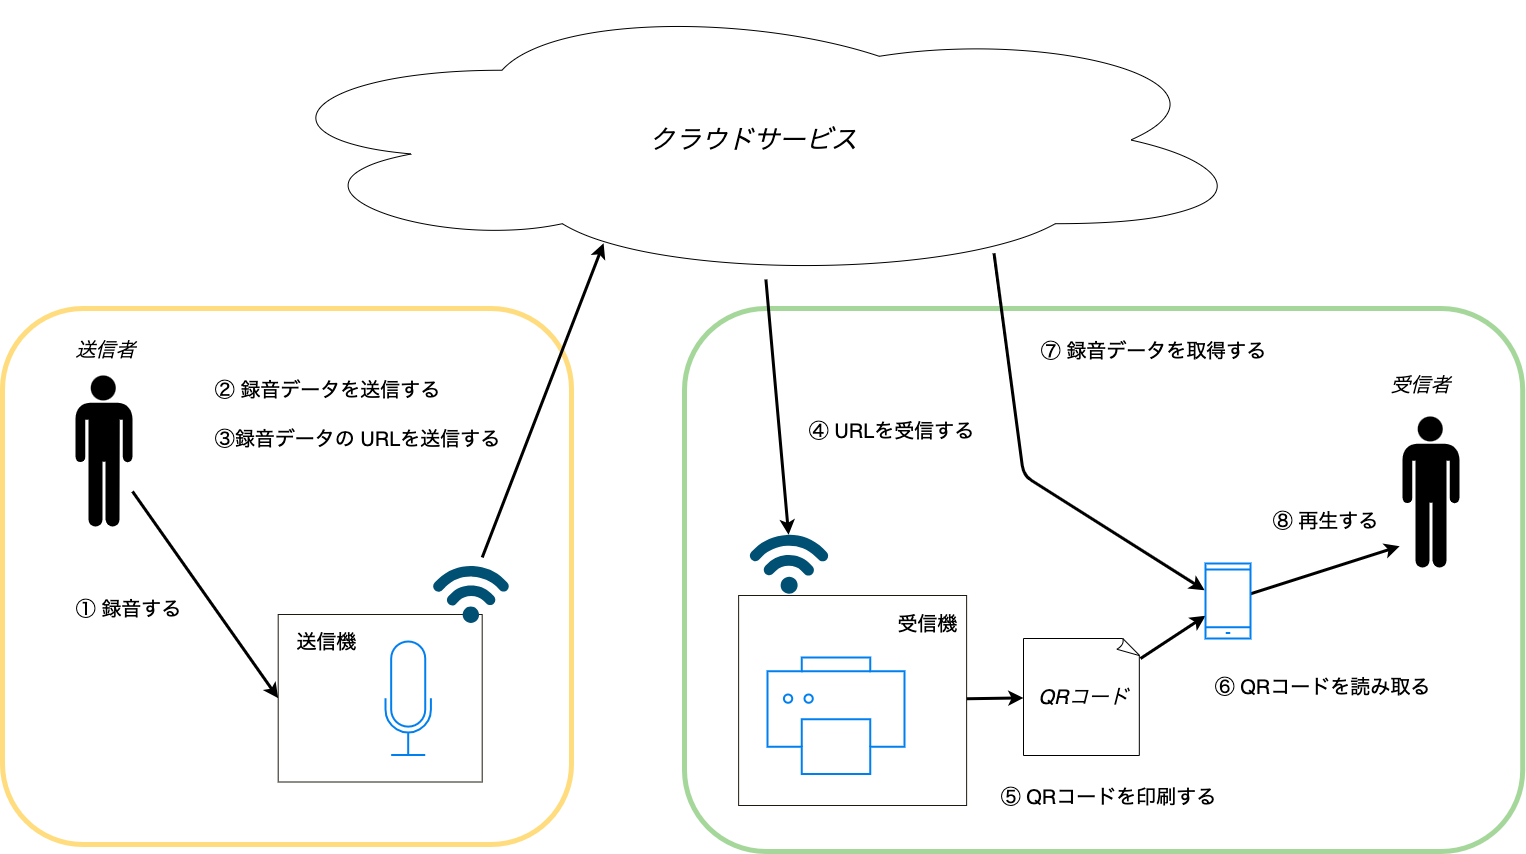
\includegraphics[scale=0.15,bb= 0 0 2000 1000]{image/system_drawio.png}
\caption{提案手法の概要図}
\label{fig:sys-overview}
\end{figure}

\subsection{ノード一覧}
本手法は大きく送信側と受信側に分けられる.
ノード一覧を\tabref{tab:sys-nodes}に示す

\begin{table}[tb] 
\caption{ノード一覧} 
\label{tab:sys-nodes}
\hbox to\hsize{\hfil
\begin{tabular}{l|l}\hline\hline
音声送信側 &	音声受信側 \\\hline
送信機 &	受信機      \\
 &	スマートフォン \\\hline
\end{tabular}\hfil}
\end{table}

\subsection{データの流れ}
\label{dataflow}
\figref{fig:sys-overview}中に,本手法におけるデータの経路を囲み数字で示した.経路は時系列順に以下のようになる.
\subsubsection*{送信側}
\begin{enumerate}
    \item 音声を録音する
    \item 録音した音声データを送信する
    \item 録音した音声データのURLを送信する 
\end{enumerate}

\subsubsection*{受信側}
\begin{enumerate}
    \item URLを受信する 
    \item URLをQRコードをに変換し,印刷する 
    \item 受信者所有のスマートフォンでQRコードを読み取る 
    \item 送信側で録音した音声データを取得する 
    \item 音声データを再生する       
\end{enumerate}


\subsection{通信プロトコル}
本手法で通信プロトコルは特に定義されないが,\ref{dataflow}中の (2)録音データの送信, (7)録音データの取得 ではHTTPが,(3)録音データへのリンクの送信, (4)リンクの受信 ではMQTTが使用されることを想定している.

\subsection{ハードウェア}
送信機受信機それぞれを構成するハードウェアの一覧を,\tabref{tab:sys-hardwares}に示す

\begin{table}[tb] 
\caption{ハードウェア一覧} 
\label{tab:sys-hardwares}
\hbox to\hsize{\hfil
\begin{tabular}{l|l}\hline\hline
送信機 &	受信機 \\\hline
MCU/MPU & MCU/MPU \\
マイクロフォン &	プリンタ \\\hline
\end{tabular}\hfil}
\end{table}

%5
\section{試作}
\ref{system}章で提案したIoTノードVoLPを,以下の観点を考慮して試作した.\figref{fig:device} \figref{fig:paper}

\begin{figure}[tb]
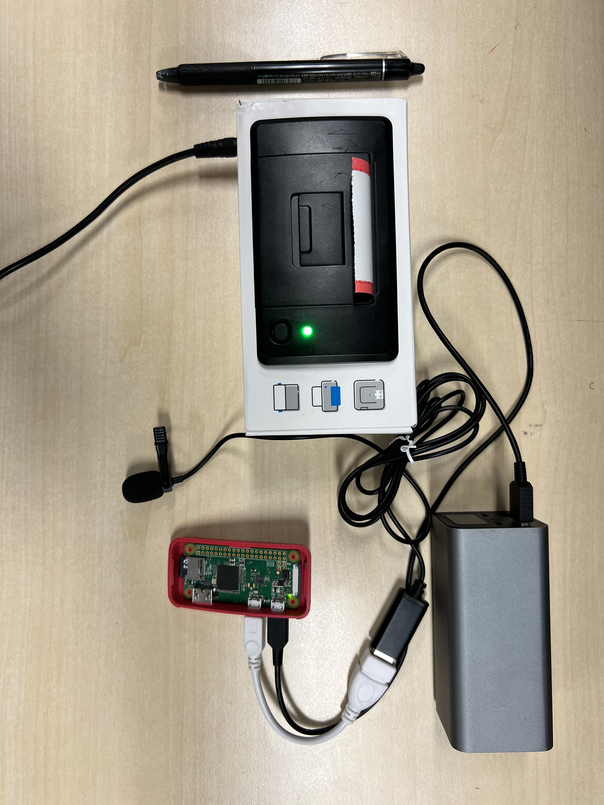
\includegraphics[scale=0.35,bb= 0 0 2000 1000]{image/device.png}
\caption{試作したIoTノード}
\label{fig:device}
\end{figure}

\begin{figure}[tb]
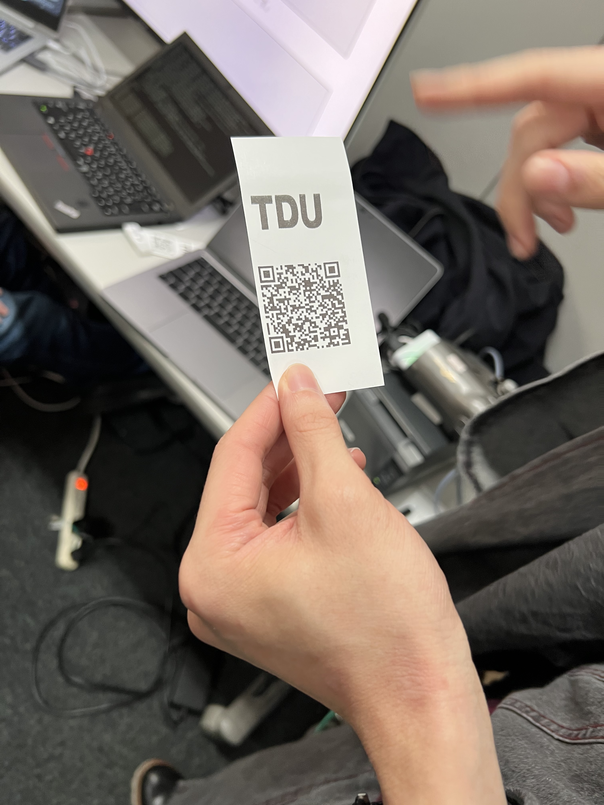
\includegraphics[scale=0.35,bb= 0 0 2000 1000]{image/paper.png}
\caption{紙に印刷したQRコード}
\label{fig:paper}
\end{figure}

本章では試作の詳細を述べる.
\begin{itemize}
    \item 屋内の電力が供給できる場所に設置することを想定
    \item 非同期コミュニケーションの場所的な自由度を高めるため,据え置き型のプリンタではなく,小型で電池駆動も可能な感熱プリンタを採用
\end{itemize}
\subsection{概要}
試作するにあたり,\figref{fig:sys-overview}をもとに具体的なノードの構成や使用するハードウェア,通信インタフェースを決定した.試作の概要図を\figref{fig:proto-overview}に示す.なお,図中のスピーカーの図柄は音声データを,図中の@は音声データのURLを示す.
\begin{figure}[tb]
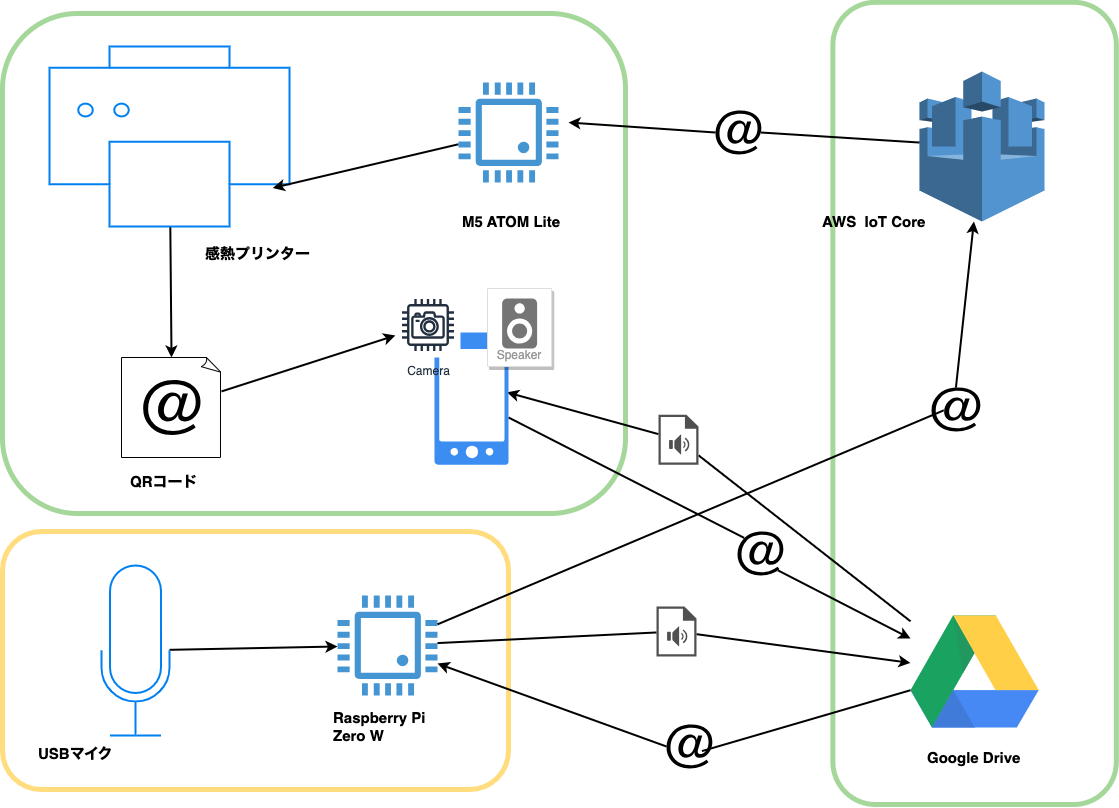
\includegraphics[scale=0.2,bb= 0 0 2000 1000]{image/proto_drawio.png}
\caption{試作物の概要図}
\label{fig:proto-overview}
\end{figure}

\subsection{ハードウェア}
試作物の送信機・受信機それぞれを構成するハードウェアの一覧を,\tabref{tab:proto-hardwares}に示す

\begin{table}[tb] 
\caption{試作物のハードウェア一覧} 
\label{tab:proto-hardwares}
\hbox to\hsize{\hfil
\begin{tabular}{l|l}\hline\hline
名称 & 用途 \\\hline
USBマイクロフォン  & 集音\\
RaspberryPi Zero W  & マイクロフォンの駆動, データの送信\\
M5 ATOM Lite  & プリンタの駆動, データの受信\\
プリンタ & QRコードの印刷\\
\end{tabular}\hfil}
\end{table}

\subsection{通信インタフェース}
試作にあたり,通信インタフェースを具体的に定義した.それらを\tabref{tab:proto-communication}にまとめる.また,表中にあるGoogleAPIは
\begin{quote}
    https://www.googleapis.com\\/upload/drive/v3/files
\end{quote}であり,アップロードへのレスポンスに含まれるJSON1の定義は\begin{quote}
    \{"kind":"drive\#file","id":"FILEID", "name":"FILENAME","mimeType":"MIMETYPE"\}
\end{quote},JSON2の定義は\begin{quote}
    \{ "link":"\$SHAREDLINK"\}
\end{quote}である.

\begin{table}[tb] 
\caption{試作物の通信インタフェース} 
\label{tab:proto-communication}
\hbox to\hsize{\hfil
\begin{tabular}{l|l|l|l}\hline\hline
用途 & プロトコル & URIなど & ペイロード\\\hline
録音 & USB & --- & WAV(F32)\\
音声アップロード & HTTP & GoogleAPI & WAV(I16)\\
レスポンス & HTTP & --- & JSON1\\
URL送信 & MQTT & volp/share/link & JSON2\\
URL取得 & MQTT & volp/share/link & WAV(F32)\\
音声取得 & HTTP & \$SHAREDLINK & ---\\
取得レスポンス & HTTP & --- & 音声データ\\
\end{tabular}\hfil}
\end{table}


%6
\section{利用シナリオの検討}
本研究のIoTノードは,音声データへのURLを紙に印刷する.これは\ref{sec:related-research}章で調査した既存の提案にはない特徴的な性質である.この性質から,本IoTノードは以下のように利用方法が拡張される
\begin{enumerate}
    \item 印刷されたQRコードの余白に手書きすることで,音声データにメタデータを後から付与できる.\\利用シナリオ: ある高齢者施設ではVoLPを活用して,入居者どうしのコミュニケーションの活性化を図っている。施設には多くの入居者がいるが,QRコードの余白にメッセージを伝えたい相手の名前を書いておくことで,迷わずに相手とやり取りができている.文字と違い音声は複数人でも聞けるので,グループ同士でも,余白にグループ名を書くことでメッセージのやりとりがある.
    \item 印刷された紙を,アノテーションしたい対象に貼り付けることで,音声が説明する対象や音声の文脈などを,現実世界に表示できる.\\利用シナリオ: 共働きの家庭で,両親は子供が起床するよりも早く外出してしまう.両親は外出する前に,VoLPで朝食の内容や朝食に付随する情報を録音して印刷し、朝食の皿の端に貼り付けておく.子供は起床後に録音を聞くが,録音内容の文脈が朝食に関するものだと一目でわかるので,録音内容をスムーズに理解することができる.両親の声を直接聞くことができ、安心して朝食を食べることができた.
    \item 印刷した紙をホワイトボードや黒板に多数貼り付けることで,スペースのかぎり,音声データを一覧できる.\\利用シナリオ: あるベンチャー企業では,VoLPを社内コミュニケーションに活用した.VoLPをオフィスに設置しておき,社員が誰でも使えるようにする.社員はその日あったできごとや,プロジェクト成功のよろこびなどを自由に印刷し,オフィスのホワイトボードに貼っていく.毎週末,ミーティング中にVoLPの振り返りの時間を設け,ホワイトボードに貼り付けられたもののなかからいくつか選んで再生することで,会社全体で進捗の喜びや課題点を共有するきっかけとなった.ホワイトボードに多数貼り付けられるという性質により,録音した回数が視覚的にわかるため,会社の活性度を図る指標にもなっている.
\end{enumerate}

%7
\section{おわりに}
本研究では,非同期コミュニケーションを促進するためのIoTノードを提案した.そして,そのプロトタイプを設計・実装した.最後に,IoTノードの利用シナリオについて検討した.本IoTノードにより,非同期音声コミュニケーションの応用範囲が広がることが期待できる.今後は,このIoTノードを一般家庭や教育施設,高齢者施設に設置し,長期実証実験を行い評価することで,有効性を検証する予定である.


\bibliographystyle{ipsjunsrt}
\bibliography{volp} 
\end{document}


